\smalltitle{سوال 2}
\begin{figure}[H]
    \centering 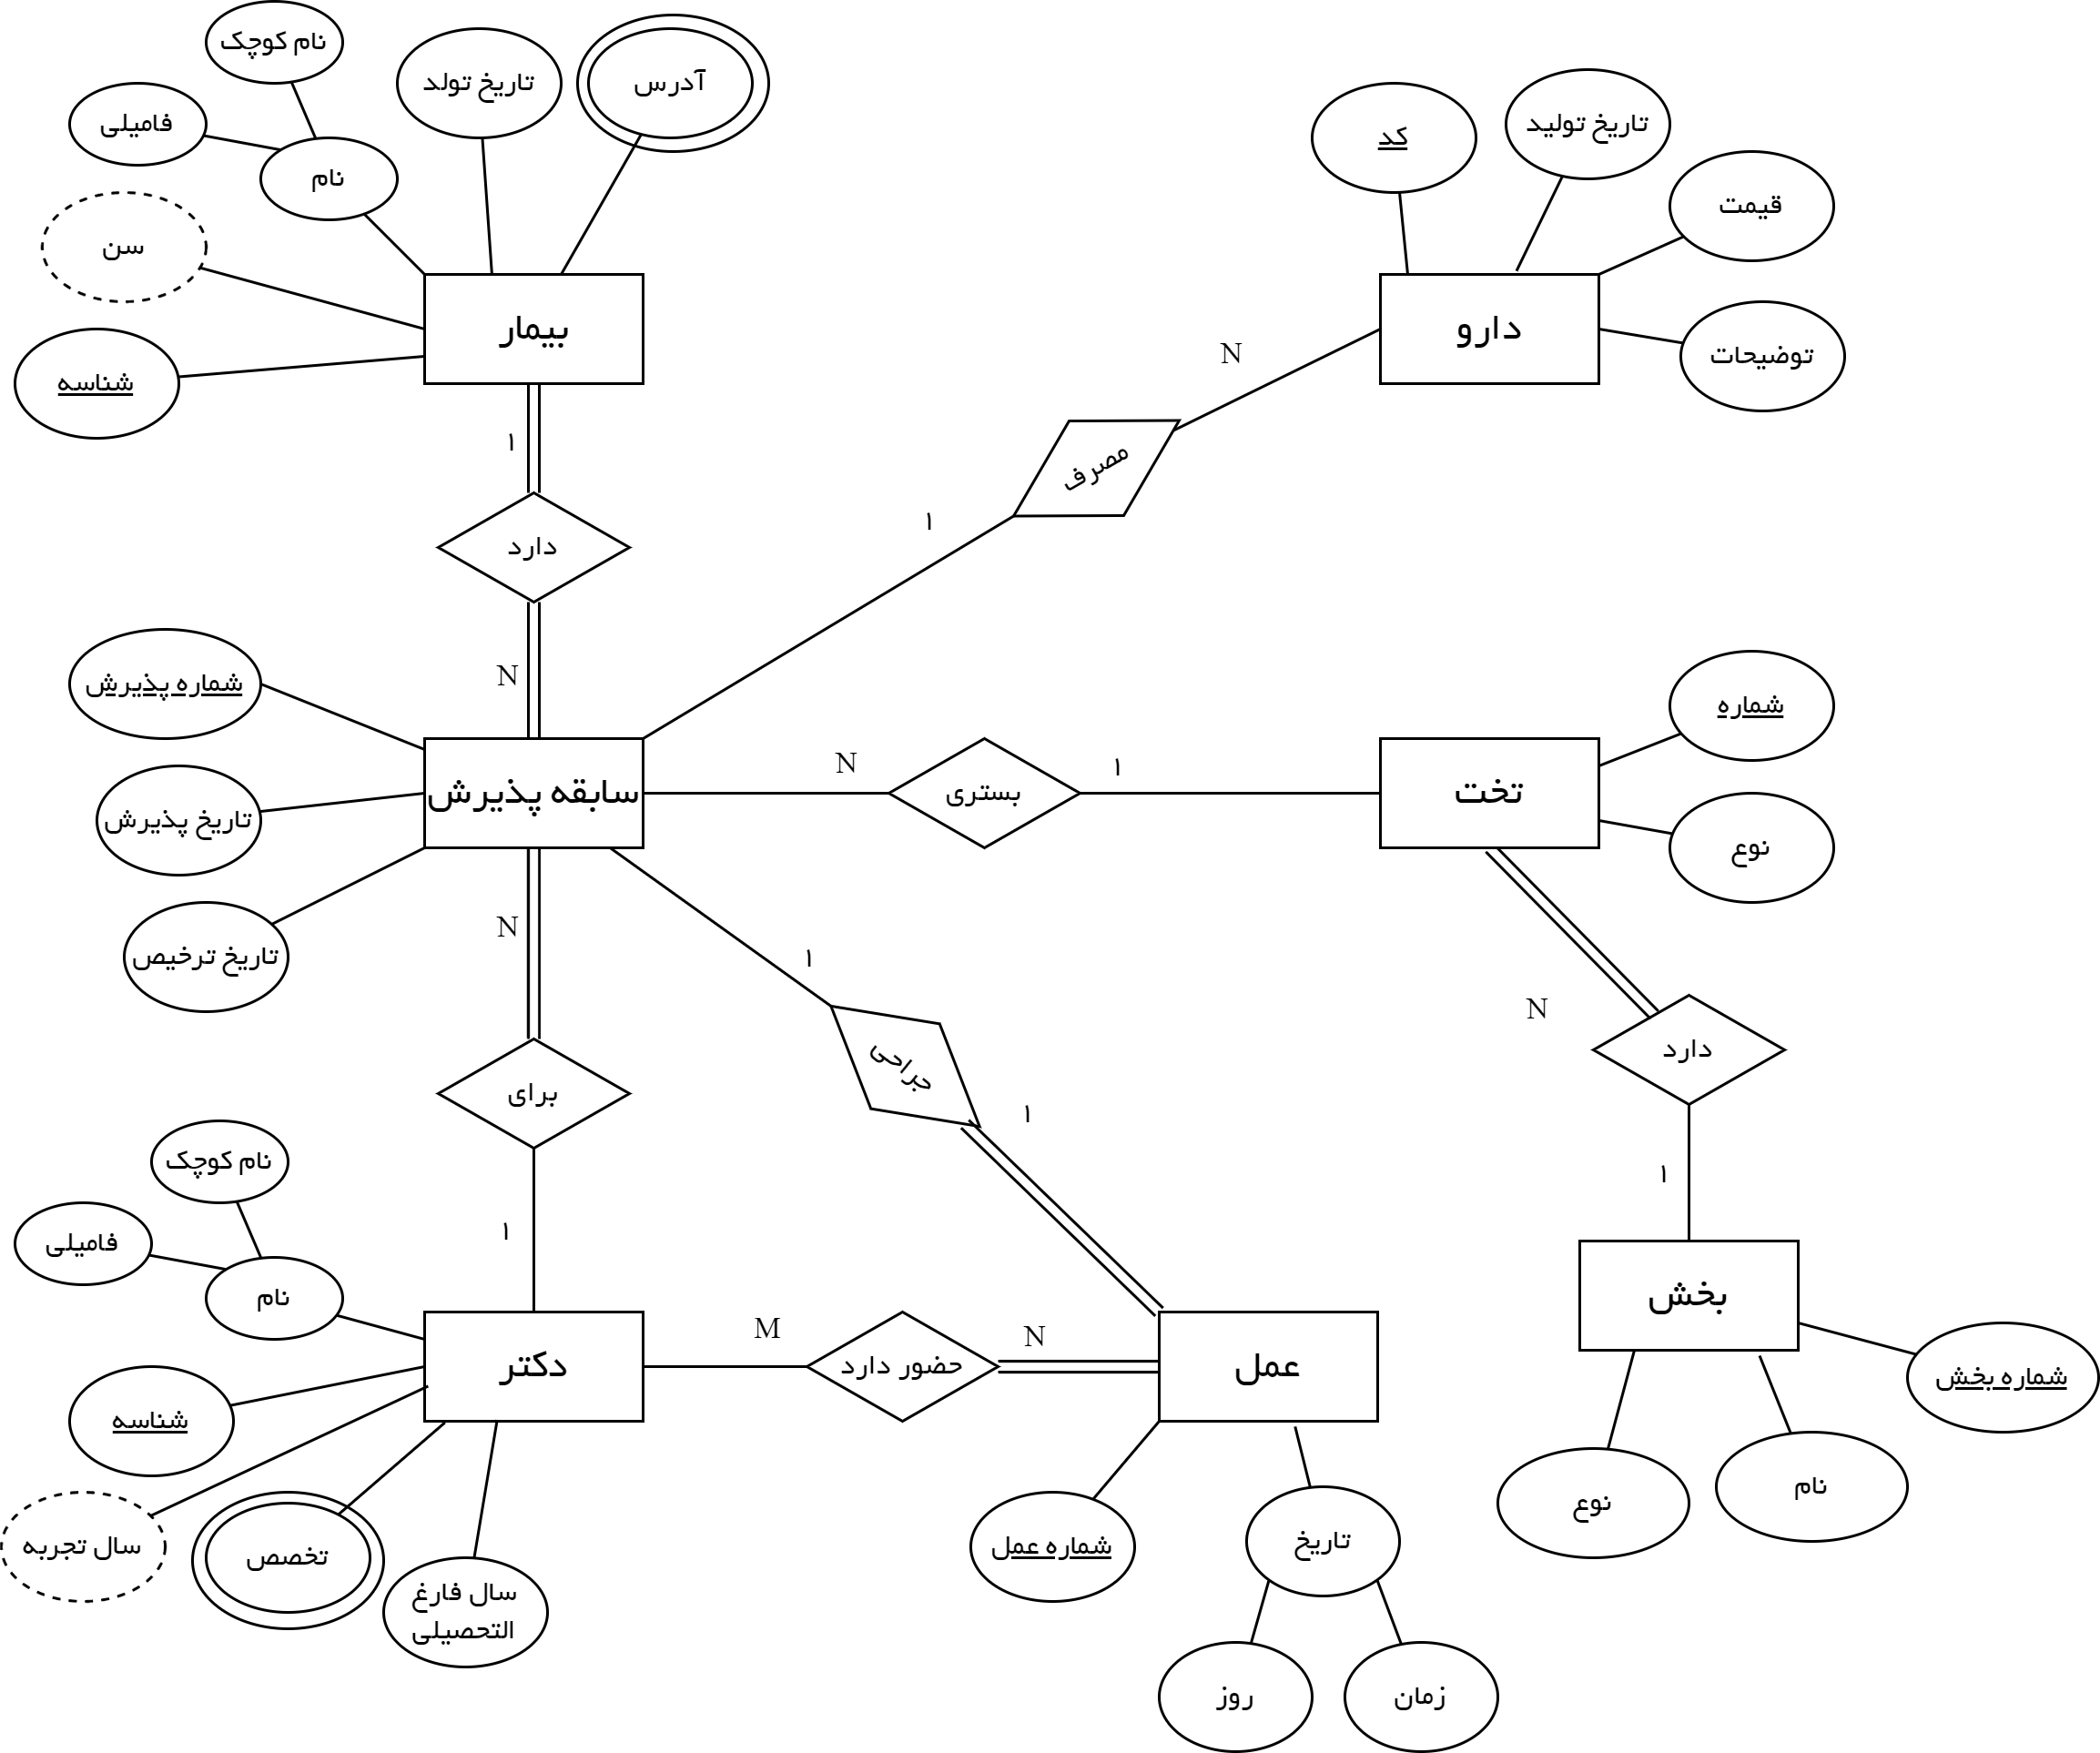
\includegraphics[scale=0.17]{pics/Hospital-ER.png}
\end{figure}
\noindent
در این مدل لازم به ذکر است که چند نکته را بیان کنم.
یکی اینکه سال تجربه‌ی دکتر با توجه به زمان فارغ التحصیلی بدست می‌آید. تا حدودی شبیه طوری که سن
از سال تولد بدست می‌آید.
همچنین مشخص است که بستری بودن، دارو، عمل و دکتر به پذیرش بیمار بر می‌گردد نه خود بیمار. همچنین فرض کرده‌ام
که زمانی که بیمار برای اولین بار وارد بیمارستان می‌شود و مشخصات خود را وارد می‌کند، پرونده‌ای برای او ساخته می‌شود.
یکی دیگر از نکاتی که به آن توجه کردم این است که احتمالا بهتر است که قسمت دارو رو به صورت زیر مدل کنیم:
\begin{figure}[H]
    \centering 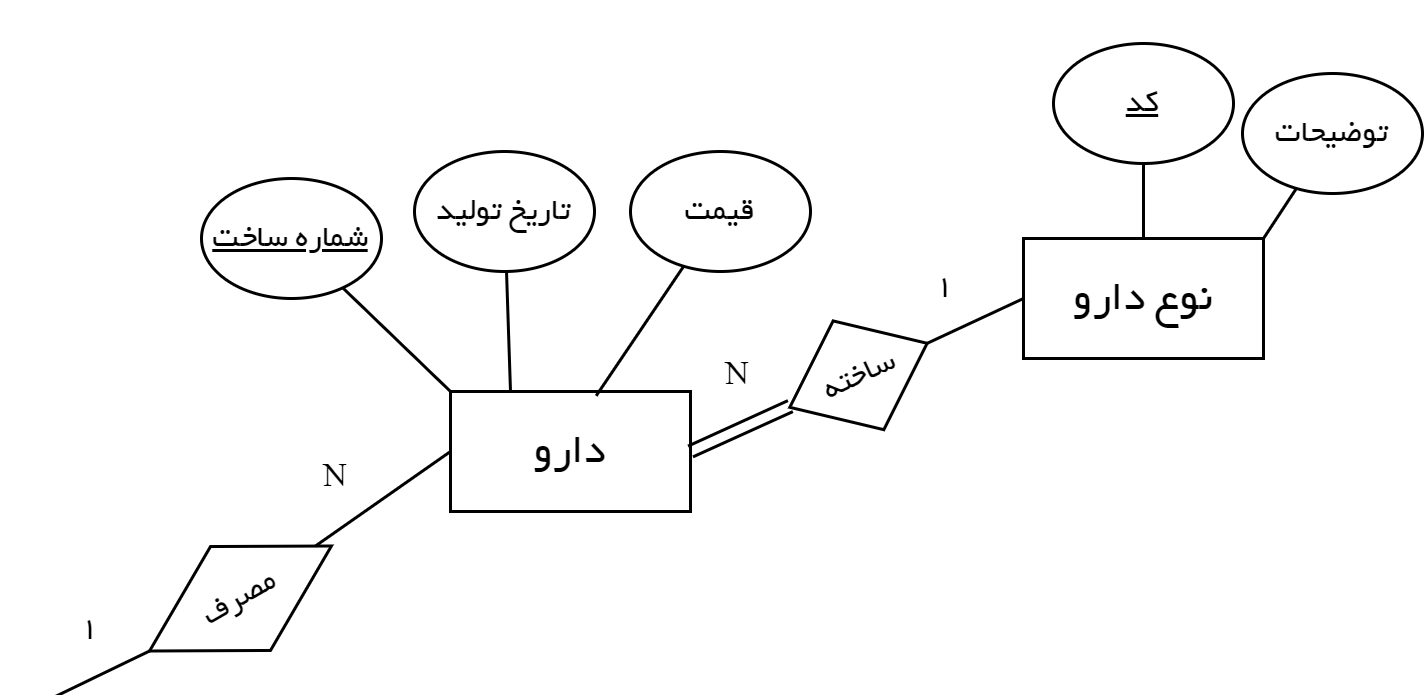
\includegraphics[scale=0.3]{pics/HospitalER-ER-Fixed.png}
\end{figure}
\noindent
دلیل این موضوع این است که کارخانه‌ای هزارتا قرص سرماخوردگی می‌سازد. تمام این قرص‌ها سرماخوردگی هستند.
اگر می‌خواستیم به صورتی که در عکس اول آمده بود قرص‌ها را ذخیره می‌کردیم کلی قرص داشتیم که در توضیحات
آنها نوشته شده بود
"سرماخوردگی"
یا چیزی متشابه با آن.
اما با این مدلسازی جدید این
\lr{duplication}
رفع می‌شود. همچنان ما می‌توانیم تورم را نیز در نظر بگیریم و قیمت دارو‌ها را کم و زیاد کنیم.

\noindent
فایل
\lr{draw.io}
این دیاگرام را می‌توانید از
\link{https://www.mediafire.com/file/pxokiauqsd39f6q/Hospital_ER.zip/file}{این}
لینک دانلود بکنید.